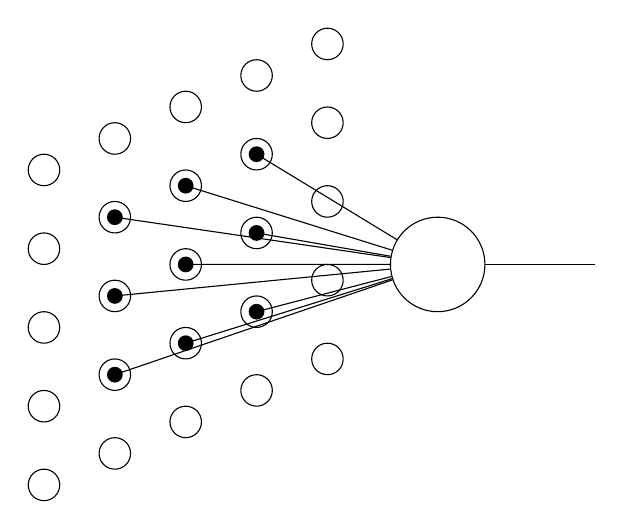
\begin{tikzpicture}
	\node[draw, circle, minimum size=1.2cm] (n) at (5,2.8) {};
	\draw (n) --  (7,2.8);
	\foreach \x in {0,1,2,3,4}
		\foreach \y in {0,1,2,3,4}
			\draw (\x*0.9+ \y*0, \x*0.4+\y*1) circle (0.2cm); %Matrixtransformation (0.7 0; 0.3 1)
	\foreach \x in {1,2,3}
		\foreach \y in {1,2,3} {
			\draw (\x*0.9+ \y*0, \x*0.4+\y*1) -- (n);
			\fill (\x*0.9+ \y*0, \x*0.4+\y*1) circle (0.1cm);
		}
\end{tikzpicture}